\section{Domain Analysis}
\phantomsection

\subsection{Problem Definition}

When designing the application, the main aim was to create a useful tool that supports the
e-learning implementation in higher educational institutions. The app should result into 
an educational instrument, that’s why, Quiz ToolKit was set to be an easy to use system 
which automates the managing of quizes with no need of expensive e-testing equipment. 
The main prerogatives of the app agenda were: quiz generation, quiz exporting, quiz scanning, 
and data processing. The problem is to accomplish these phases. 

The first one, quiz generation, deals with the direct interaction of the human (our case 
lecturer) with the technology (QTK). The academic staff is naturally reluctant to change their 
methods of teaching and learning without a deep understanding of why and how and what 
will be the impact in terms of quality and any resultant benefits. That is why it was 
important to make the app able to offer the users various options for quiz 
generation. Another important point was to keep the interface simple, at the same time 
easy to understand and use. Important to notice, that the final form of the quiz contains 
not only the quiz text, but distinctive reference markers (circles) and a QR code. These are 
essential for the successive phases. The markers should serve as location references and 
QR codes should store the id of each copy and the current page of the generated quiz copy.

Quiz exporting represents the phase when the quizes are getting a physical shape. The 
questions/answer keys previously introduced manually by lecturer and organized 
automatically into single/individual quizes by the app are being printed out in hard 
copies. The format should meet the printing requirements, be readable and clear. 

The third issue, quiz scan, implies the use of a scanner. For hundreds of quizes there is a 
need of a fast scanner that can quickly and accurate process the hard copies of the tests. 
An important point is the scan quality on which depends the next phase: data . 

The final issue, data analyzing, is completely automatic. In this phase the app should process 
the information using the elements added to the quiz pages earlier. The program should use the 
reference marks to depict correct the position of the answers, in case of scan inaccuracy (page rotation and translation) and read the QR code to collect the copy data. Also, an evaluation criteria should be developed 
in order to get an instant feedback of the results.

\subsection{REST}
REST (Representational State Transfer) relies on a stateless, client-server architecture that uses the HTTP protocol in the most cases.
REST is an architecture style used in the development of Web services. Instead of using complex mechanisms such as CORBA, RPC or SOAP to connect between devices, REST is preffered as a way for the devices to communicate.
REST uses HTTP for the CRUD operations (Table \ref{crud_operations}).
\begin{table}[ht!]
\centering
\caption{CRUD operations}
{
\renewcommand{\arraystretch}{1.25}
\begin{tabular}{ lll }

  Operation & SQL & HTTP \\ \hline
  Create &  INSERT & PUT/POST \\
  Read(Retrieve) & SELECT & GET \\
  Update(Modify) & UPDATE & PUT/PATCH \\
  Delete(Destroy) & DELETE & DELETE \\

\end{tabular}
}
\label{crud_operations}
\end{table}

As a programming approach, REST is a lightweight alternative to Web Services.
A REST service is:
\begin{itemize}
  \item Does not depend on platforms (the server can be Unix, Mac or any other kind)
  \item Based on standards (runs on top of HTTP)
  \item Is not language dependent(Java can communicate with Python)
  \item Can be easily used if there are firewalls present
\end{itemize}

There are six constraints which describe the REST architecture. Five of them are mandatory. If the system doesn't comply with these, it cannot be considered RESTful, even though it is constructed in a RESTlike way.
These are the six constraints that define the RESTful architecture style:
\begin{enumerate}
  \item Uniform Interface

    The \textit{uniform interface} constraint simplifies and declutches the architecture into parts, which can then grow independently. It represents the interface between clients and servers. The uniform interface is an essential part of the outline of any REST services.  The rules which direct the uniform interface are:

    \begin{description}
      \item[Resource-Based] \hfill \\
        URIs are the resource identifiers, which help to detect the individual resources in a request. The resources and the representations, that are returned to the client as an answer to their request are two considered two separate things. As an example, the server sends some database records in a XML or JSON, which can be expressed in different languages and encodings, based on the server implementation and the particularity of the received request, instead of sending its database.

      \item[Manipulation of Resources Through Representations] \hfill \\
        If a client has the permission to modify or delete a resource on the server, he can do so, given he has a representation of that resource and the metadata it holds, if any.

      \item[Self-descriptive Messages] \hfill \\
        Messages must contain sufficient information, so the hosts know how to process them. Given a media type in the message, the host will choose the necessary parser to operate on the contents of it. Responses must explicitly mention if they are cacheable.

      \item[Hypermedia as the Engine of Application State (HATEOAS)] \hfill \\
        State is delivered between hosts via hypermedia. Clients provide state through body contents, query parameters, request headers and the resource name (URI). Servers endow state to clients via response codes, headers and body content.
        HATEOAS also expresses the possibility of placing the URI in the body or header of the response to provide the resource name for the recovery of the relevant objects.
    \end{description}

  \item Stateless

    The \textit{statelessness} of the REST architecture signify that the request contains the required state, which is used to deal with the request itself.
    It can be inside the URI, query-string parameters, body or headers. The resource is identified by the URI and its state is found in the body. The request is analized and processed by the server and then the according state is transmitted back via response body, headers.
    In REST, the server does not have to preserve, update or transmit the session state, thus allows more scalability. Session state is stored fully on the client. The client must contain in the request all the information for the server, so it can be performed. Also including state if it should spread more requests.

    The application state is the data used for the current session or request by the server, to carry out a request. A resource is the data that represents the resource description, which can be the data that is stored in the database. The application state can differ per request and client, where the resource state remains the same for every client that sends a request for it.

    This constraint establishes visibility, reliability, and scalability. The system doesn't have to look at anything else besides the request itself to identify the character of the request, thus improving visibility. The recuperation from small errors is easier, making the system more reliable. The server doesn't need to administer resource usage of requests and to store state from requests, which makes the system easier to maintain and develop.

  \item Cacheable

    The clients must have the possibility to \textit{cache} responses. To avert clients reutilizing outdated or deficient data in requests, the responses must declare themselves as cacheable or non-cacheable. Scalability and performance can be enhanced, when caching is adequately managed, thus decreasing certain client-server communication and reducing the average latency. 

  \item Client-Server

    \textit{Clients and servers} are divided by the uniform interface. This means that the portability of the client code can be increased by leaving, for example, the data storage to the responsibility of the server, making the client unrelated dircectly with the storage mechanism. Servers also are improved by this splitting by making it ignorant to the user state or interface, thus making them more intelligible and scalable. Given that the interface is not intefered with, servers and clients can be extended and changed without taking care of any diret relation between them.

  \item Layered System

    Intermediary serevers are used in a \textit{layered system}. They can improve the system's scalability by using load-balancing of services between multiple networks and shared caches. Also, the security can be strenghtened by the use of layers. Clients should not be able to differentiate whether it is connected directly to the server it is accessing or to an intermediate server.
    The downside of a layered system is that it can generate overhead and latency to the data processing. If it is supports cache contstraints, then it can profit from the shared caching at intermediary servers.

  \item Code on Demand (optional)

    The functionality of the client side can be enhanced by providing executable logic by the servers. The amount of features to be implemented at client-side drops thanks to this constraint. System extensibility is improved by having the opportunity to download additional features to the system.

\end{enumerate}

If we support these constraints, we get the following possibilities inside our system:
\begin{itemize} 
  \item Scalability
  \item Simplicity
  \item Modifiability
  \item Visibility
  \item Portability
  \item Reliability
\end{itemize}


\subsection{Rails}

Rails has some principles to which it adheres to:
\begin{description}

  \item[Don't Repeat Yourself] DRY says that ``Every piece of knowledge must have a single, unambiguous, authoritative representation within a system.'' \cite{dry_principle} You can get more maintainability and extensibility by refraining to write duplicate code, documentation or any other information related to the system being developed. 

  \item[Convention Over Configuration] ``Rails has opinions about the best way to do many things in a web application, and defaults to this set of conventions, rather than require that you specify every minutiae through endless configuration files.'' \cite{rails_principles}

  \item[Fat models, skinny controller] The main application logic must be placed inside the model. The controller must remain as thin as possible. 
\end{description}


Rails is a web-application framework that includes all necessary to create web applications fitting to the Model-View-Controller (MVC) pattern.
MVC pattern comprehension is essential to understanding Rails, so MVC will be described further. 
Figure \ref{rails_mvc} shows how Rails implements MVC. 

\begin{figure}[!ht]
\centering
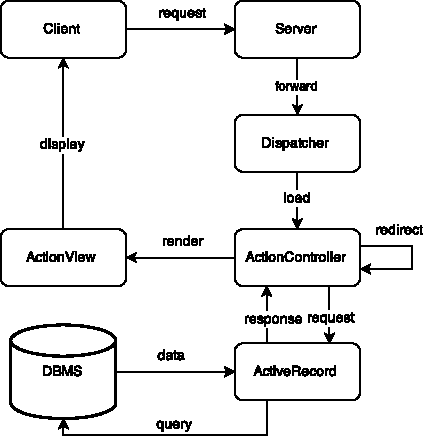
\includegraphics[scale=1.2]{rails_MVC}
\caption{Rails MVC}\label{rails_mvc}
\end{figure}

MVC splits your application into three layers, each having a distinctive duty.

The Model layer depicts your domain model and contains the business logic that is individual to your application. ActiveRecord::Base is the class from which the database-backed model classes are inherited, in Rails. Data from database tuples are given as objects which have business logic methods, thanks to Active Record. Models can be ordinary Ruby classes, or classes that apply a set of interfaces as given by the Active Record module, while most Rails models are supported by a database.

Incoming HTTP requests and the appropriate responses for them are managed by the Controller layer.
Rails controllers can generate HTML, XML, JSON, mobile views, PDFs as returning response to the request. Controllers render view templates and control the models so that it can give a suitable HTTP response. 

Action Dispatch parses the web request's contained information routes the requests to the right controller and deals with advanced processing connected to HTTP:
\begin{itemize}
  \item MIME-type negotiation
  \item Decoding parameters in PUT, PATCH and POST
  \item Control HTTP caching, cookies and sessions
\end{itemize}

Controller classes inherit from the ActionController::Base class and implement actions to manage requests. The content which is generated from views is usually what is displayed as the result of an action. 

In Rails framwork, the Action Dispatch functionality is dispatched by default, and the users interface with the Action Controller module, which prompts the Action View rendering. 

Action Pack contains both Action Dispatch and Action Controller modules. So it provides both the view and the controller layers of the MVC. Action Pack is a framework that manages web requests. With it, you can route (map the request URLs to their respective actions), establish controllers which apply actions, and render views(templates of different formats) as responses.

``Templates'' are the essential part of the View layer and they are the ones that deliver the  proper representations of the app's resources. The most frequent view temlates are ERB files, which are HTML with embedded Ruby, though they can be found in diverse formats. Action View manages the view generation. A controller response or some text is usually rendered in a view.
 
Rails also has Action Mailer, used to generate and send emails; Active Job, an interface used to put different jobs to run on background using one of the queueing backends; Active Support, a module offering library extensions and utility classes.

The jobs that \textit{Active Job} declare are anything that needs processing, code that need to be split in smaller tasks and run in parallel, code that takes to much time for the user to wait, sending mails and others. 

Action Mailer's $\#deliver\_later$ method, that transforms the email sending process into a background job that will be executed later is supported by Active Job as its backend. Mailing in background is basic in today's web applications, freeing the user from waiting for the server's response in order to proceed further.
  
Active Job provides a job insfrastructure for every Rails application, in both background and immediate processing options. Other backend libraries for creating background jobs can be added to the system and there is no need to worry about the differences in the API in these libraries. Also this gives the possibility to change them without having to write your jobs anew.




\subsection{Quick Response Codes}
The QR code, which stands for Quick Response Code, is a two-dimensional barcode, which was initially used for tracking inventory. It was developed in Japan by a subdivision of Toyota. Today, it is widely spread and people have found more and more uses for it. The fast gain in popularity was due to the superiority of the QR codes’ read speed and storage capacity versus the UPC barcodes.

The QR code is  composed of black square dots placed on a white square background. It is usually read by a phone camera, which has a QR decoding software. The code image is then interpreted and the data is extracted.

The code can be read from any direction in 360 degree. The three corners of the QR code contain the positional detecting patterns, which make this thing possible.

\subsubsection{QR Error Correction}
The QR error correction is used to restore the data on a damaged code. There are four levels of correction. If a higher level is set, the error correction is more efficient but less characters can be encoded. So you must be careful when deciding which error correction level to use. Most of the time, the decisive factor is the environment in which the QR codes will be used. So take the probability of the QR code to be damaged into consideration and decide about the error correction level accordingly.

\subsubsection{QR code sizes}
The black dots in the code are also called modules. Their size are an important factor that categorize the QR codes in readable and not readable by certain devices. The QR codes become unreadable if their modules’ size are below the resolution limitation of the imaging device’s camera.

The QR code is designed in such a way that, the more data you want to store in it, the more columns and rows containing modules will be inserted. Therefore, a QR code must have a bigger size when a larger amount of data is encoded and vice-versa.

So, the QR codes have been categorized in versions, from Version 1 to Version 40.  QR code Versions differing from the previous one by having 4 more modules on each side: Version 1 with ( 21 x 21 modules ) with possibility of storing 25 alphanumerics with the lowest correction level and Version 40 with  ( 177 x 177 modules ) with 1852 alphanumerics. The maximum data storage for each version is derived from the amount of data, character type and correction level.


\begin{figure}[!ht]
  \centering
  \subfloat[Version 1 QR code\label{fig1.1a}]{%    
    
\includegraphics[width=0.48\textwidth,natheight=292, natwidth=292]{qr_v1.png}    
  }
 \hspace{0.09cm}
  \subfloat[Version 40 QR code\label{fig1.1b}]{%
    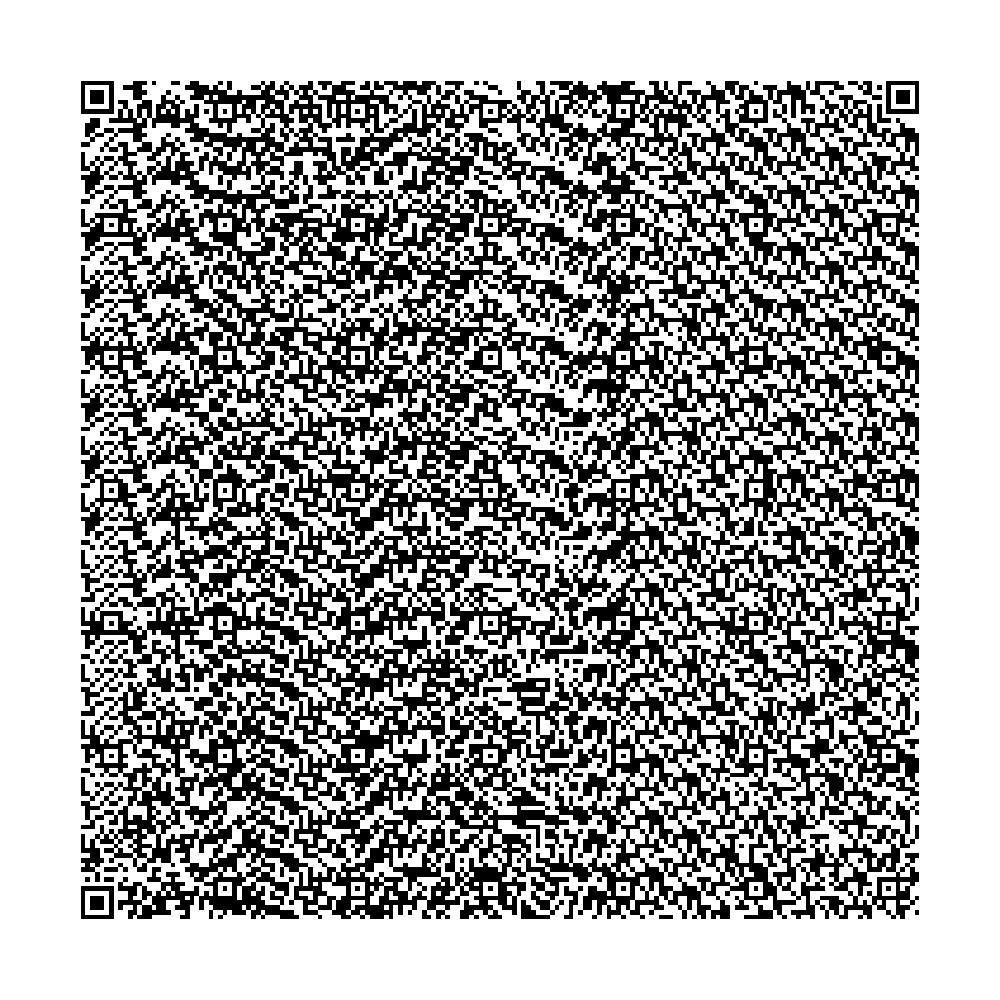
\includegraphics[width=0.48\textwidth,natheight=1000, natwidth=1000]{qr_v40.png}
  }
  \caption{Version 1 QR code with 21 x 21 modules (a), version 40 QR code with 177 x 177 modules (b).}
  \label{fig1.1}
\end{figure}

Having this technology at hand, the system gets to simplify the way in which it recognizes the different pages it is processing at the low level of its implementation. Given that information being stored in the QR code will be minimal, it is not required a size bigger than the Version 1 provides us, thus saving some space on the printed paper. The correction level will be set to high, for safety reasons and also because it won’t conflict with the number of characters needed to be encoded.

\newpage
\subsection{Tesseract}


\subsection{Prawn}
Prawn is a PDF generation library written in ruby that is simple to use, quite performant and provides features such as:

\begin{itemize} 
  \item PDF builtin and embedded TrueType fonts support.
  \item Vector drawing, for objects as lines, curves, ellipses, polygons, rectangles.
  \item Inserting PNG and JPG images, with scaling options.
  \item PDF outlines for navigation support.
  \item Password protection and encryption.
  \item Basic layout low level tools, grid system.
  \item Allows users to make custom extensions.
  \item Extensive text rendering for flowing text.
  \item Content iteration rendering for page numbers, footers and headers.
  \item Support for UTF-8 fonts encoding, fallback font, right to left text rendering, internationalization features and customizable text wrapping.
\end{itemize}

Prawn is not a HTML to PDF generator. It is also not used for publishing or reporting. It is a particularly adaptable PDF document generation system. 

The special characteristic which differentiate Prawn from other systems is that the origin of the page is considered the botom left corner. This thing makes it a bit unconvenient when using Prawn alongside a system which has the origin situated at the top left corner. Still, the page is filled from the top to the bottom, thus the cursor for inserting content starts at the top of the page. After the content is entered, the functions responsible for putting it in, proceed to the page's bottom.

PDF Documents are generated in three different ways:
\begin{enumerate}
  \item Prawn::Document instance creation
    \begin{lstlisting}[language=Ruby, caption={Prawn Document generation with instance creation}, label=ruby_prawn1]
    pdf = Prawn::Document.new
    pdf.text "New document"
    pdf.render_file "document.pdf"
    \end{lstlisting}

  \item Using Prawn::Document.generate method
    \begin{lstlisting}[language=Ruby, caption={Prawn Document generation with method}, label=ruby_prawn2]
    Prawn::Document.generate("document2.pdf") do 
      text "generate without block argument"
    end
    \end{lstlisting}

  \item The generate method with explicit block arguments
    \begin{lstlisting}[language=Ruby, caption={Prawn Document generation with block argument}, label=ruby_prawn3]
    Prawn::Document.generate("document3.pdf") do |pdf|
      pdf.text "generate with block"
    end
    \end{lstlisting}
\end{enumerate}

When we create the instance object of Prawn::Document, we have to call $render\_file$ to generate the pdf document. 
When using the generate method, the pdf object will be rendered after the block has been exited. When no block argument is given, a freshly created Prawn::Document instance is used for evaluating the block. When the block argument is given, a instance is created and passed to the block. The implicit method is preferred, because it requires less typing and defines and renders the pdf at the same time. 


\subsection{Image Processing}

\subsubsection{Chunky PNG}

ChunkyPNG is a Ruby library, which hasn't got any dependency on any other libraries, thus being a plain Ruby library.
It has the following features:

\begin{itemize}
  \item Read/Write access to the image’s pixels.
  \item Alpha formation of different images.
  \item Supports all color modes (grayscale, true color and indexed) and transparency. Based on the image’s colors, the most suitable color mode will be chosen automatically
  \item Decodes all PNG standard images. This means that all standard color modes with variable depth of the bits and transparency, filtering options are also contained in Chunky PNG.
  \item For images that are stored in chunks, you get Read/Write acess to all its metadata.
  \item There is the possibility to operate with RMagick.
  \item Depending on the device, it uses an integer number of bytes of memory for every pixel, making it memory efficient.
  \item By only using integer math and an encoding routine, it is considered quite fast for Ruby norms. 
\end{itemize}

PNGs can be loaded from files, IO streams and binary string:

\begin{lstlisting}[language=Ruby, caption={Loading PNGs with Chunky PNG}, label=chunky_png1]
File.open('image.png', 'rb') do |input| 
  png = ChunkyPNG::Image.from_io(input)
end
png = ChunkyPNG::Image.from_file('image.png')
png = ChunkyPNG::Image.from_blob(File.read('image.png'))
\end{lstlisting}

Consider supplying the pixel data as a raw RGBA or RGB formatted stream, because the decoding fo PNG files is really slow and because, loading these types of streams will be \~1000 faster than loading the PNG encoded image.

\begin{lstlisting}[language=Ruby, caption={Loading pixel stream with Chunky PNG}, label=chunky_png2]
png = ChunkyPNG::Image.from_rgba_stream(width, height, File.read('pixels.rgba'))
png = ChunkyPNG::Image.from_rgb_stream(width, height, File.read('pixels.rgb'))
\end{lstlisting}

The image data can be saved and encoded to a file, IO stream or binary string:
\begin{lstlisting}[language=Ruby, caption={Loading pixel stream with Chunky PNG}, label=chunky_png3]
png.save('file.png')
File.open('iostream.png', 'wb' ) do |io| 
  png.write(io)
end
binary_string = png.to_blob
\end{lstlisting}

The weakness of ChunkyPNG is that it is vulnerable to DOS attacks. When loading a certain constructed PNG file, ChunkyPNG can run out of memory. It is very hard to apply a fix due to the pure-Ruby character of the library. To avoid this issue and reliably deal with images that are not to be trusted, the image processing done by ChunkyPNG must be done in a different process.


\subsubsection{Oily PNG}
ChunkyPNG can be sped up using the OilyPNG Ruby C extension. OilyPNG does not require any libraries because it is an independent module. It has a different approach to encoding and decoding PNG images than ChunkyPNG's. The implementation of these operations is much faster.

Performance comparison in tables \ref{decoding_speed} and \ref{encoding_speed} cited from \cite{encode_decode_speed}:

\begin{table}[ht!]
\centering
\caption{Decoding speed in seconds}
{
\renewcommand{\arraystretch}{1.25}
\begin{tabular}{ lll }
                        &  ChunkyPNG   &  OilyPNG   \\ \hline
PNG - no filtering      & 1.056832   & 0.078345 \\
PNG - UP filtering      & 3.327986   & 0.078387 \\
PNG - PAETH filtering   & 7.499367   & 0.089143 \\
From RGBA pixelstream   & 0.032571   & 0.035790 \\
From RGB pixelstream    & 0.221163   & 0.226358 \\
\end{tabular}
}
\label{decoding_speed}
\end{table}

\begin{table}[ht!]
\centering
\caption{Encoding speed in seconds}
{
\renewcommand{\arraystretch}{1.25}
\begin{tabular}{ lll }
                        & ChunkyPNG   &   OilyPNG \\ \hline
Autodetect (indexed)    & 1.762275    & 0.715871 \\
$:no_compression$       & 0.999972    & 0.704999 \\
$:fast_rgba$            & 0.279853    & 0.098239 \\
$:fast_rgb$             & 0.285781    & 0.071865 \\
$:good_compression$     & 1.015139    & 0.717544 \\
$:best_compression$     & 3.809578    & 0.713787 \\
$:rgb$                  & 2.603707    & 0.084677 \\
$:rgba$                 & 3.451300    & 0.114356 \\
$:indexed$              & 1.799546    & 0.707457 \\
$:interlaced$           & 1.778964    & 0.715108 \\
to RGBA pixelstream     & 0.242787    & 0.250338 \\
to RGB pixelstream      & 0.257684    & 0.264674 \\
\end{tabular}
}
\label{encoding_speed}
\end{table}



\subsection{Resque}
Some work can't be done instantly and needs to be scheduled for another time. Resque can be used to do this in a simple way and also gives you the possibility to manage all the work that the application had stacked.
Resque is a library for creating background jobs and it uses Redis to manage the queues. The created jobs can be put on multiple queues and processed at a later time.
Any Ruby class or module that responds to the $perform$ method, can be a background job. Classes can be created with intention to do background jobs, or the already existing classes can be converted as jobs.

Resque contains three parts:

\begin{enumerate}
  \item A Ruby library for creating, processing and querying jobs
  \item A Rake task for starting a worker for job processing
  \item A Sinatra application for keeping track of the jobs, queues and workers.
\end{enumerate}

Resque workers assigned to different devices, they can uphold priorities and are resistant against memory leaks. They indicate what they're doing and expect failure.

Resque queues are always available, deliver visibility into their internals and stack the jobs as JSONs. Also, thanks to Redis, Redis queues support atomic push and pop.

What workers work on or don't work on, what queues they are operating in, what's inside those queues, is shown by the Resque frontend. It also offers usage stats, and helps tracking errors.

To do some background work, a job must be defined with a $work$ method, as in listing \ref{job_define}:

\begin{lstlisting}[language=Ruby, caption={Defining a job class}, label=job_define]
class FileProcessingJob
  def work
    # Processing a file
  end
end
\end{lstlisting}

Further, we need to put our job on the queue \ref{job_enqueue}:

\begin{lstlisting}[language=Bash, caption={Enqueue a job}, label=job_enqueue]
queue = Resque.new
queue << FileProcessingJob.new
\end{lstlisting}

Now, this job will be enqueued in Redis. We just need a worker to get it and work on it \ref{worker_start}:
\begin{lstlisting}[language=Bash, caption={Create a worker}, label=worker_start]
$ bin/resque work
\end{lstlisting}

The process that is started here, queries the Redis queue, takes any job that is there and executes it. This process repeats itself over and over again. The ``--queue'' option can be used to specify the queue from which the worker should take his jobs. The ``--interval'' option is used to give waiting time before the worker polls the queue for a new job.

Workers react to several signals:
\begin{enumerate}
  \item QUIT - Wait for child process to end then exit
  \item TERM / INT - Instantly kill child process then exit
  \item USR1 - Instantly kill child process but don't exit
  \item USR2 - No jobs are started being processed
  \item CONT - After USR2 signal start processing jobs again
\end{enumerate}

QUIT signal is usually used to shutdown a worker.
If an obsolete or clogged child need to be killed, USR1 should be used. If the child is present, the processing will continue as normal. Otherwise the parent process is shut down, because Resque is going to see it as a bad process.
To kill an obsolete or clogged child and shutdown, TERM should be used.
To leave the worker running, but not doing any jobs, USR2 is used to stop the processing. CONT is used to restart it.


Jobs can be anything that isn't fast enough to be waited upon in the main application interface. These things are various and there is always something that can be safely run as a background job.
\begin{itemize}
  \item Deleting data from database
  \item Computing disk usage
  \item Building tarballs
  \item Populate cache with valid data
  \item Building graphs
  \item Generating stuff
  \item Creating events in the db and pre-caching them
\end{itemize}

The queues' priority indicate which one will be processed first. When all of the jobs from a higher priority queue are processed and there is none left, the jobs from a lower priority queue are going to be executed.

The ``queue list'' is the list containing the queues put in the order given by the user. Resque does not have numeric priorities, so this ``queue list'' is used instead. 

When we add a $high\_priority$ queue near the $medium\_priority$ queue, the worker is started using rake, like this \ref{two_queues_worker}:
\begin{lstlisting}[language=Bash, caption={Working on two queues}, label=two_queues_worker]
$ QUEUES=high_priority,medium_priority rake resque:work
\end{lstlisting}

The $high\_priority$ queue is first checked when searching for jobs. If the worker finds a job on this queue, it starts processing it and then check this queue again. This repeats until no job is found. Now, the next queue, which is $medium\_priority$ will be queried for jobs. If a job is found, the worker will process it and then check again the highest priority queue. In this way the queues are prioritized in Resque.


\clearpage

